#import "@local/bootlin:0.1.0": * 

#import "@local/bootlin-yocto:0.1.0": *

#import "@local/bootlin-utils:0.1.0": *

#import "../../typst/local/themeBootlin.typ": *

#import "../../typst/local/common.typ": *

#show: bootlin-theme.with(
  aspect-ratio: "16-9",
config-common(
  handout: "handout" in sys.inputs and sys.inputs.handout == "1",
))

#show raw.where(block: true): set block(fill: luma(240), inset: 1em, radius:0.5em, width:100\%) 

#show raw.where(block: false): r => { text(fill: color-link)[#r] } 

#show raw.where(lang: "c", block: true): r => \{

set block(fill: luma(240),
inset: 0.4em,
radius: 0.5em,
width: 95\%, breakable: true, above: 12pt, below: 12pt)

set text(11pt)

r

\} 


#show raw.where(lang: "console", block: true): r => \{

set block(fill: luma(240),
inset: 0.4em,
radius: 0.5em,
width: 95\%, breakable: true, above: 6pt)

set text(100pt)

r

\} 

 === [fragile]{strace}
  
#columns(gutter: 8pt)[
  \small
  System call tracer - \url{https://strace.io}
  \begin{itemize}
  \item Available on all GNU/Linux systems\\
        Can be built by your cross-compiling toolchain generator or by your build system.
  \item Allows to see what any of your processes is doing: accessing files, allocating memory...
        Often sufficient to find simple bugs.
  \item Usage:\\
    `strace <command>` (starting a new process)\\
    `strace -f <command>` ({\bf f}ollow child processes too)\\
    `strace -p <pid>` (tracing an existing process)\\
    `strace -c <command>` (time statistics per system call)
    `strace -e <expr> <command>` (use {\bf e}xpression for advanced filtering)
  \end{itemize}
  See \href{https://man7.org/linux/man-pages/man1/strace.1.html}{the strace
      manual} for details
   #colbreak()
  \includegraphics[height=0.7\textheight]{common/strace-mascot.png}\\
  \tiny Image credits: \url{https://strace.io/}
  \\]


=== [fragile]{strace example output}
  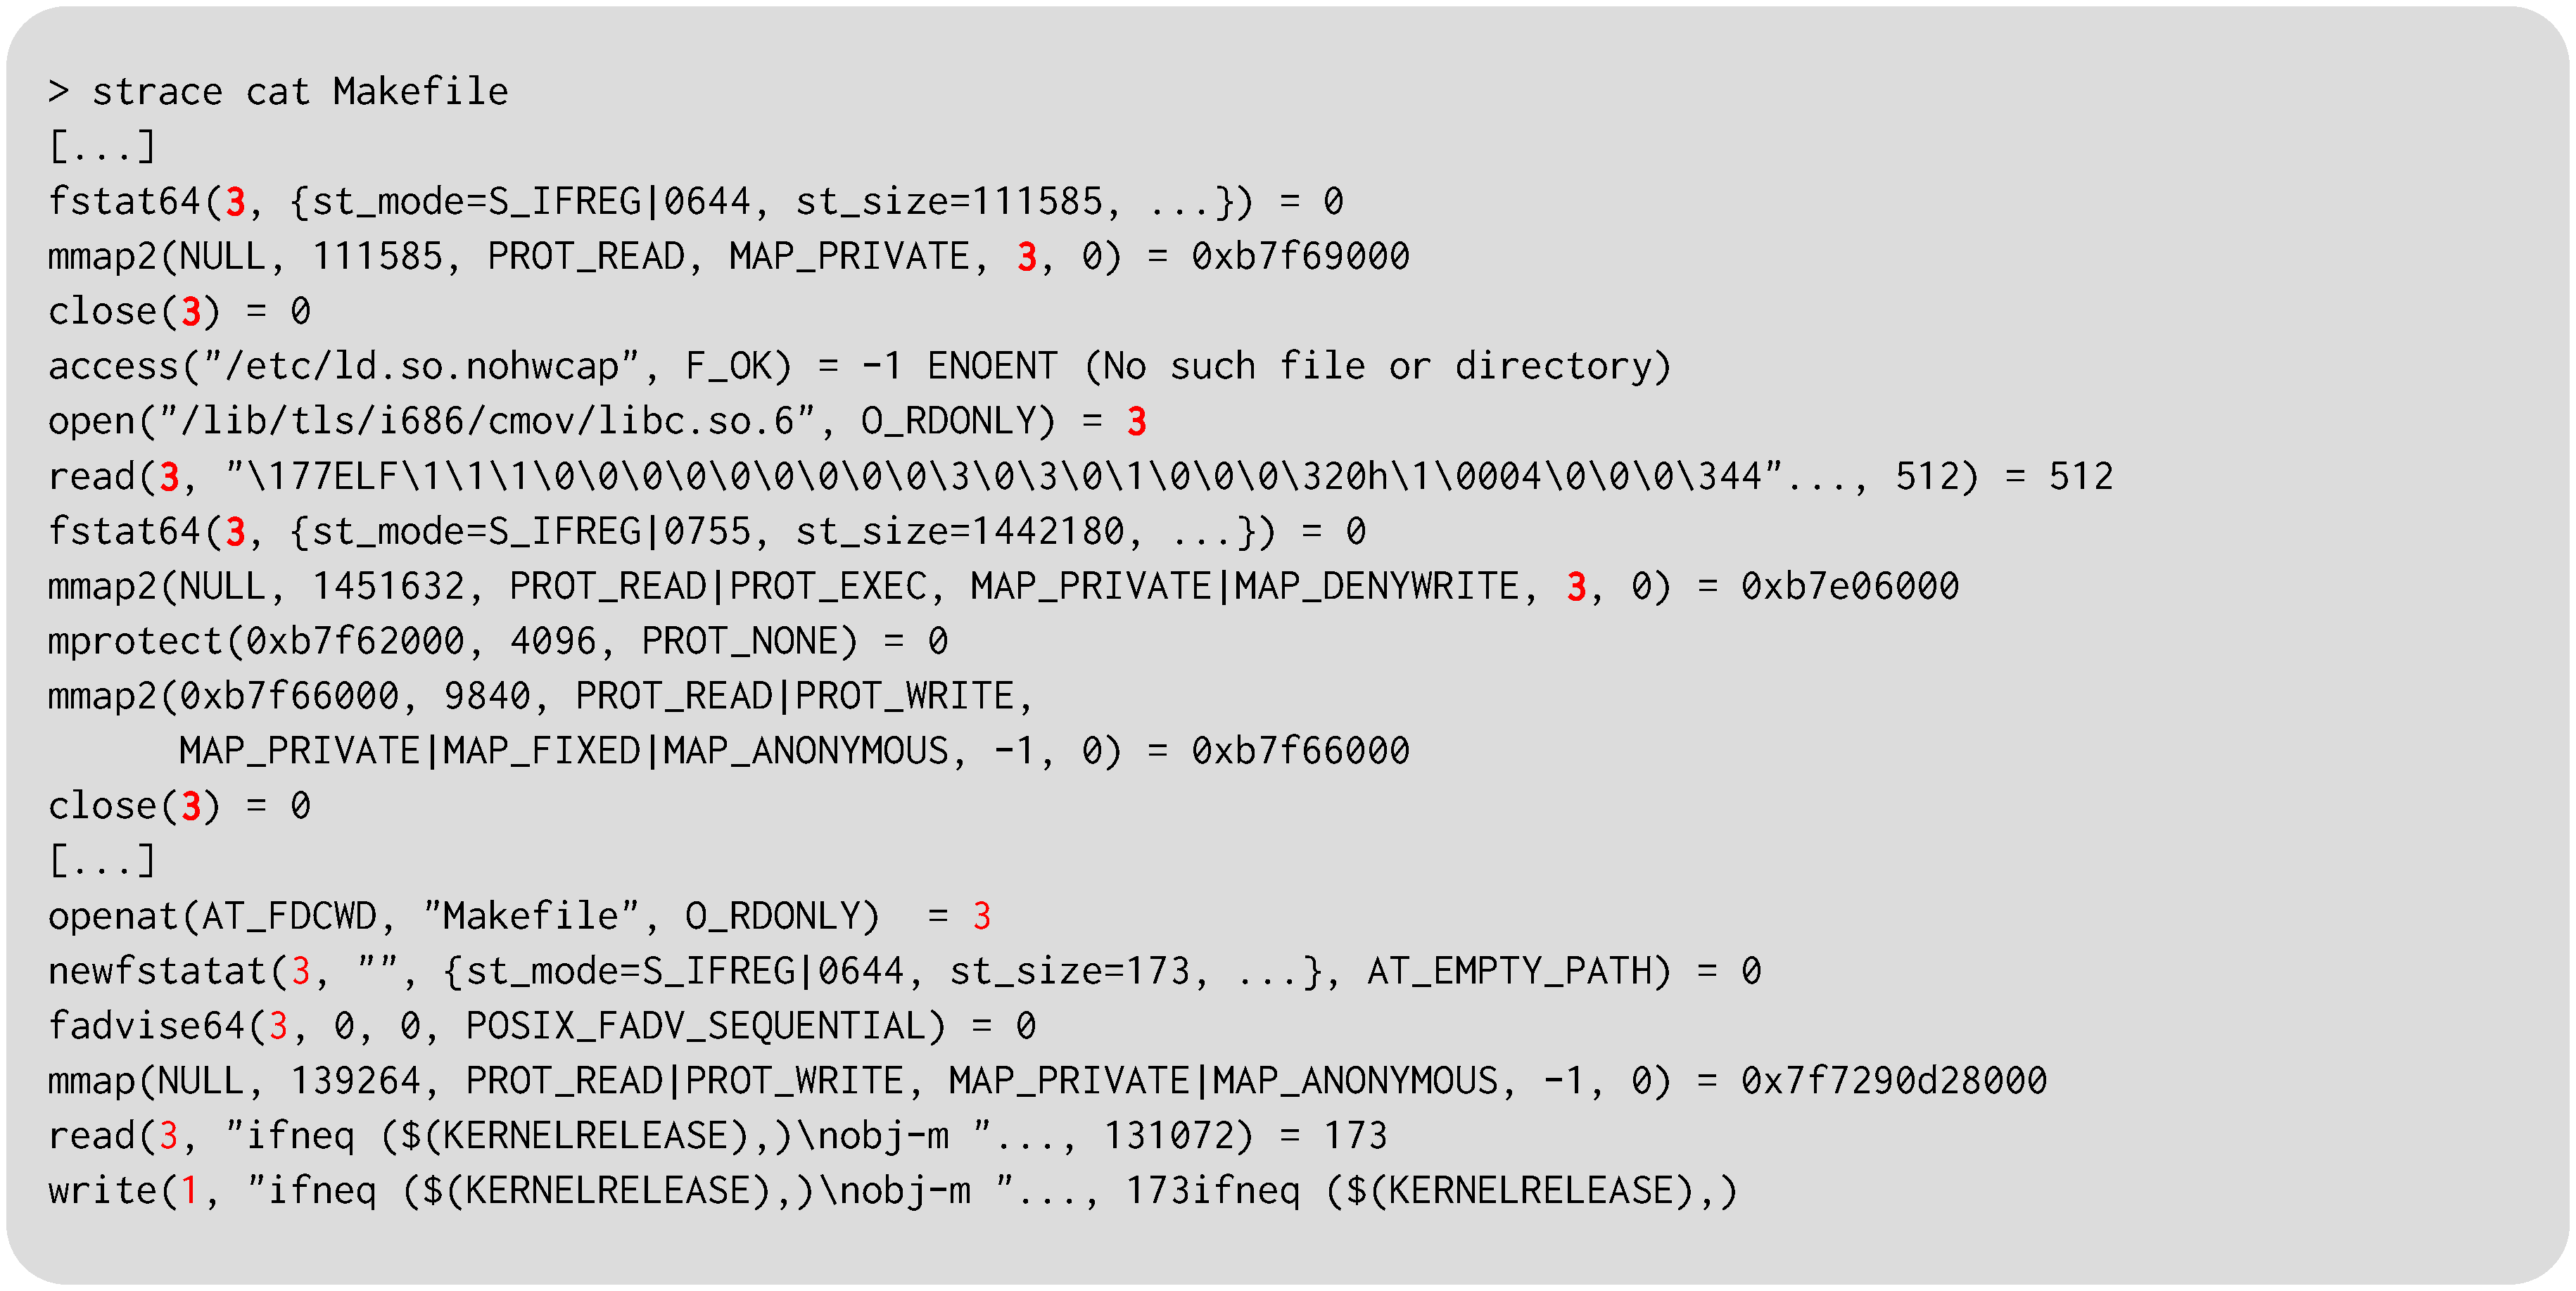
\includegraphics[height=0.75\textheight]{common/strace-output.pdf}\\
  Hint: follow the open file descriptors returned by `open()`.
  This tells you what files are handled by further system calls.


=== [fragile]{strace filtering }
  \begin{itemize}
  \item Display only a specific set of system calls:
  \end{itemize}
  \begin{block}{}
    \begin{minted}[fontsize=\scriptsize]{console}
$ strace -e 'openat,write' cat Makefile
    \end{minted}
  \end{block}
  \begin{itemize}
  \item Filter out specific system calls:
  \end{itemize}
  \begin{block}{}
    \begin{minted}[fontsize=\scriptsize]{console}
$ strace -e '!poll' cat Makefile
    \end{minted}
  \end{block}
  \begin{itemize}
  \item Show only system calls returning a specific status
  \end{itemize}
  \begin{block}{}
    \begin{minted}[fontsize=\scriptsize]{console}
$ strace -e 'status=failed' cat Makefile
    \end{minted}
  \end{block}
  \begin{itemize}
  \item Trace how a file is accessed and used among different system calls
  \end{itemize}
  \begin{block}{}
    \begin{minted}[fontsize=\scriptsize]{console}
$ strace -P '/etc/ld.so.cache' cat Makefile
    \end{minted}
  \end{block}
  \begin{itemize}
    \item Run `strace --tips` to learn new commands !
  \end{itemize}

